%%% Settings %%%%%%%%%%%%%%%%%%%%%%%%%%%%%%%%%%%%%%%%%%%%%%%%%%%%%%%%%%%%%%%%%%%%%%%%%
\documentclass{article}

\usepackage{graphicx}  % serve per inserire immagini
\usepackage{fancyhdr}  % creazione header-footer
\usepackage{tabularx}  % serve per creare tabelle con colonne a larghezza variabile
\usepackage{ifthen}  % serve per mostrare cose diverse in base a condizioni
\usepackage{geometry}
\usepackage{setspace}
\usepackage{tikz}
\usepackage[italian]{babel}
\usepackage[hidelinks]{hyperref}
\usepackage{pgfgantt}  % per i diagrammi di Gantt
\usepackage{eurosym}
\usepackage{float}
\usepackage{longtable}


% setta a 1 se il verbale è esterno, 0 se è interno
\newcommand{\isEsterno}{1}

% Margini della pagina
\geometry{a4paper, margin=1in}

% Intestazione personalizzata
\pagestyle{fancy}
\fancyhf{}
\fancyhead[L]{Code7Crusaders - Software Development Team}
\fancyhead[R]{\thepage}

% Spaziatura delle righe
\setstretch{1.2}

\begin{document}
\setcounter{secnumdepth}{5} % Permette la numerazione fino a \subparagraph
%%%%%%%%%%%%%%%%%%%%%%%%%%%%%%%%%%%%%%%%%%%%%%%%%%%%%%%%%%%%%%%%%%%%%%%%%%%%%%%%%%%%%%



%%% Sezione del titolo %%%%%%%%%%%%%%%%%%%%%%%%%%%%%%%%%%%%%%%%%%%%%%%%%%%%%%%%%%%%%%%
\begin{titlepage}

    \AddToHookNext{shipout/background}{
        \begin{tikzpicture}[remember picture,overlay]
        \node at (current page.center) {
            
\includegraphics{../../img/background.png}
        };
        \end{tikzpicture}
    }

    \centering
    \vspace*{2cm}
    
    
\includegraphics[width=0.3\textwidth]{../../img/logo/7Crusaders_logo.png} % logo
    \vspace{1cm}
    
    {\Huge \textbf{Code7Crusaders}}\\
    \vspace{0.5cm}
    {\Large Software Development Team}\\
    \vspace{2cm}
    
    {\large \href{https://code7crusaders.github.io/docs/RTB/documentazione_interna/glossario.html#piano-di-progetto}{\textbf{Piano di Qualifica}\textsuperscript{G}}}\\
    \vspace{5cm}
    
    
    \textbf{Membri del Team:}\\
    Enrico Cotti Cottini, Gabriele Di Pietro, Tommaso Diviesti \\
    Francesco Lapenna, Matthew Pan, Eddy Pinarello, Filippo Rizzolo \\
    \vspace{0.5cm}
    
    \vspace{1cm}
\end{titlepage}
%%%%%%%%%%%%%%%%%%%%%%%%%%%%%%%%%%%%%%%%%%%%%%%%%%%%%%%%%%%%%%%%%%%%%%%%%%%%%%%%%%%%%%



% Versioni %%%%%%%%%%%%%%%%%%%%%%%%%%%%%%%%%%%%%%%%%%%%%%%%%%%%%%%%%%%%%%%%%%%%%%%%%%%
% \newpage
\begin{table}[h!]
\centering
\textbf{Versioni} \\ % Titolo sopra la tabella
\vspace{2mm} % Spazio tra il titolo e la tabella
\begin{tabular}{|c|c|c|c|c|}
    \hline
    \textbf{Ver.} & \textbf{Data} & \textbf{Autore} & \textbf{Verificatore} & \textbf{Descrizione} \\
    \hline
    1.0 & 10/02/2025 & Gabriele Di Pietro & Filippo Rizzolo & Approvazione documento \\
    0.5 & 06/02/2025 & Gabriele Di Pietro & Matthew Pan & Stesura sezione 3.2 \\
    0.4 & 20/01/2025 & Matthew Pan & Filippo Rizzolo & Stesura sezione 3.1 - Test Sistema \\
    0.3 & 16/12/2024 & Gabriele Di Pietro & Matthew Pan & Stesura sezione 5 \\
    0.2 & 10/12/2024 & Gabriele Di Pietro & Francesco Lapenna & Aggiunte tabelle \\
    0.1 & 05/12/2024 & Gabriele Di Pietro & Enrico Cotti Cottini & Prima stesura del documento \\  
    \hline
\end{tabular}
%\caption{Versioni del documento}
\label{tab:versioni}
\end{table}
%%%%%%%%%%%%%%%%%%%%%%%%%%%%%%%%%%%%%%%%%%%%%%%%%%%%%%%%%%%%%%%%%%%%%%%%%%%%%%%%%%%%%%
\newpage


% Indice %%%%%%%%%%%%%%%%%%%%%%%%%%%%%%%%%%%%%%%%%%%%%%%%%%%%%%%%%%%%%%%%%%%%%%%%%%%%%
% \newpage
\tableofcontents
\listoftables
\listoffigures
%%%%%%%%%%%%%%%%%%%%%%%%%%%%%%%%%%%%%%%%%%%%%%%%%%%%%%%%%%%%%%%%%%%%%%%%%%%%%%%%%%%%%%



% Sezione Introduzione %%%%%%%%%%%%%%%%%%%%%%%%%%%%%%%%%%%%%%%%%%%%%%%%%%%%%%%%%%%%%%%
\newpage
\section{Introduzione}
\subsection{Obiettivo del Documento}
Il documento ha lo scopo di definire le strategie di verifica e validazione per assicurare il corretto funzionamento e uno standard di qualità
dello strumento sviluppato e delle attività che lo accompagnano. Sarà sottoposto a revisioni continue, così da poter seguire l'evoluzione del progetto.

\subsection{Glossario}
Il \href{https://code7crusaders.github.io/docs/RTB/documentazione_interna/glossario.html#glossario}{Glossario\textsuperscript{G}} è uno strumento utilizzato per risolvere eventuali dubbi su termini specifici utilizzati nella redazione del documento. Esso conterrà la definizione dei 
termini evidenziati e sarà consultabile al seguente \href{https://code7crusaders.github.io/docs/RTB/documentazione_interna/glossario.html}{link}. I termini presenti in tale documento
saranno evidenziati da una 'G' al pedice.

\subsection{Riferimenti}
\subsubsection{Normativi}
\begin{itemize}
    \item \textbf{Regolamento del progetto} \\ \texttt{\url{https://www.math.unipd.it/~tullio/IS-1/2024/Dispense/PD1.pdf}}
    \item \textbf{Norme del Progetto} \\ \texttt{\url{https://code7crusaders.github.io/docs/RTB/documentazione_interna/norme_di_progetto.html}}
\end{itemize}
\subsubsection{Informativi}
\begin{itemize}
    \item \textbf{Standard ISO/IEC 25010} \\ \texttt{\url{https://iso25000.com/index.php/en/iso-25000-standards/iso-25010}}
    \item \textbf{Standard ISO/IEC 12207:1995} \\ \texttt{\url{https://www.math.unipd.it/~tullio/IS-1/2009/Approfondimenti/ISO_12207-1995.pdf}}
    \item \textbf{Qualità di prodotto} \\ \texttt{\url{https://www.math.unipd.it/~tullio/IS-1/2024/Dispense/T07.pdf}}
    \item \textbf{Qualità di processo} \\ \texttt{\url{https://www.math.unipd.it/~tullio/IS-1/2024/Dispense/T08.pdf}}
    \item \textbf{Verifica e validazione}
    \begin{itemize}
        \item Introduzione \\ \texttt{\url{https://www.math.unipd.it/~tullio/IS-1/2024/Dispense/T09.pdf}}
        \item Analisi Statica \\ \texttt{\url{https://www.math.unipd.it/~tullio/IS-1/2024/Dispense/T10.pdf}}
        \item Analisi Dinamica \\ \texttt{\url{https://www.math.unipd.it/~tullio/IS-1/2024/Dispense/T11.pdf}}
    \end{itemize}
    \item \textbf{Capitolato d'appalto C7} \\ \texttt{\url{https://www.math.unipd.it/~tullio/IS-1/2024/Progetto/C7.pdf}}
    \item \textbf{Verbali esterni ed interni} \\ \texttt{\url{https://code7crusaders.github.io/docs/RTB/index.html}}
    \item \textbf{Analisi dei requisiti} \\ \texttt{\url{https://code7crusaders.github.io/docs/RTB/documentazione_esterna/analisi_dei_requisiti/analisi_dei_requisiti.html}}
    \item \href{https://code7crusaders.github.io/docs/RTB/documentazione_interna/glossario.html#glossario}{\textbf{Glossario}\textsuperscript{G}} \\ \texttt{\url{https://code7crusaders.github.io/docs/RTB/documentazione_interna/glossario.html}}
\end{itemize}
\newpage
\section{Metriche di qualità}
La qualità di processo è un criterio fondamentale ed è alla base di ogni prodotto che
rispecchi lo stato dell’arte. Per raggiungere tale obiettivo è necessario sfruttare delle
pratiche rigorose che consentano lo svolgimento di ogni attività in maniera ottimale.
Al fine di valutare nel miglior modo possibile la qualità del prodotto e l’efficacia dei
processi, sono state definite delle metriche, meglio specificate nel documento Norme
di ProgettoG e qui di seguito riepilogate. Esse sono state suddivise utilizzando lo \textbf{Standard \texttt{ISO/IEC12207:1995}}, il quale separa i processi di ciclo di vita del software in processi di
base e/o primari, processi di supporto e processi organizzativi.
\subsection{Processi di base e/o primari}
\subsubsection{Fornitura} %Tabella
\begin{table}[H]
    \centering
    \renewcommand{\arraystretch}{1.5} % Aumenta lo spazio tra le righe
    \begin{tabular}{|c|l|c|c|}
        \hline
        \textbf{Codice} & \textbf{Nome} & \textbf{Ammissibile} & \textbf{Ottimale} \\
        \hline
        1PBM-PV & \href{https://code7crusaders.github.io/docs/RTB/documentazione_interna/glossario.html#planned-value}{Planned Value\textsuperscript{G}} & $PV \geq 0$ & $PV \leq BAC$ \\
        2PBM-ETC & Estimated to Complete & $ETC \geq 0$ & $ETC \leq EAC$ \\
        3PBM-EAC & Estimated at Completion & $EAC \leq BAC + 10\%$ & $EAC \leq BAC$ \\
        4PBM-EV & \href{https://code7crusaders.github.io/docs/RTB/documentazione_interna/glossario.html#earned-value}{Earned Value\textsuperscript{G}} & $EV \geq 0$ & $EV \leq EAC$ \\
        5PBM-AC & \href{https://code7crusaders.github.io/docs/RTB/documentazione_interna/glossario.html#actual-cost}{Actual Cost\textsuperscript{G}} & $AC \geq 0$ & $AC \leq EAC$ \\
        6PBM-SV & \href{https://code7crusaders.github.io/docs/RTB/documentazione_interna/glossario.html#scheduled-variance}{Scheduled Variance\textsuperscript{G}} & $SV \geq -10\%$ & $SV \geq 0\%$ \\
        7PBM-CV & \href{https://code7crusaders.github.io/docs/RTB/documentazione_interna/glossario.html#cost-variance}{Cost Variance\textsuperscript{G}} & $CV \geq -10\%$ & $CV \geq 0\%$ \\
        8PBM-CPI & Cost Performance Index & $CPI \geq 0.8$ & $CPI \geq 1$ \\
        9PBM-SPI & Scheduled Performance Index & $SPI \geq 0.8$ & $SPI \geq 1$ \\
        10PBM-OTDR & On-Time Delivery Rate & $OTDR \geq 90\%$ & $OTDR \geq 95\%$ \\
        \hline
    \end{tabular}
    \label{tab:fornitura}
    \caption{Metriche di qualità per il processo di Fornitura}
\end{table}
% \newpage

\subsubsection{Sviluppo} %Non inserire nulla
\paragraph{Analisi dei requisiti}%Tabella
\textbf{(11PBM - 13PBM)}

\begin{table}[H]
\centering
\renewcommand{\arraystretch}{1.5} % Aumenta lo spazio tra le righe
\begin{tabular}{|c|l|c|c|}
    \hline
    \textbf{Codice} & \textbf{Nome} & \textbf{Ammissibile} & \textbf{Ottimale} \\
    \hline
    11PBM-PRO & Percentuale Requisiti Obbligatori & $PRO = 100\%$ & $PRO = 100\%$ \\
    12PBM-PRD & Percentuale Requisiti Desiderabili & $PRD \geq 30\%$ & $PRD = 100\%$ \\
    13PBM-PRF & Percentuale Requisiti Facoltativi & $PRF \geq 0\%$ & $PRF = 100\%$ \\
    \hline
\end{tabular}
\label{tab:analisi_requisiti}
\caption{Metriche di qualità per il processo di Analisi dei requisiti}
\end{table}
\newpage
\paragraph{Progettazione}%Tabella
\textbf{(14PBM)}
\begin{table}[H]
    \centering
    \renewcommand{\arraystretch}{1.5} % Aumenta lo spazio tra le righe
    \begin{tabular}{|c|l|c|c|}
        \hline
        \textbf{Codice} & \textbf{Nome} & \textbf{Ammissibile} & \textbf{Ottimale} \\
        \hline
        14PBM-PG & Profondità delle Gerarchie & $PG \leq 7$ & $PG \leq 5$ \\
        \hline
    \end{tabular}
    \label{tab:progettazione}
    \caption{Metriche di qualità per il processo di Progettazione}
\end{table}
\paragraph{Implementazione}%Tabella
\textbf{(15PBM - 18PBM)}
\begin{table}[H]
    \centering
    \renewcommand{\arraystretch}{1.5} % Aumenta lo spazio tra le righe
    \begin{tabular}{|c|l|c|c|}
        \hline
        \textbf{Codice} & \textbf{Nome} & \textbf{Ammissibile} & \textbf{Ottimale} \\
        \hline
        15PBM-PPM & Parametri per Metodo & $PPM \leq 7$ & $PPM \leq 5$\\
        16PBM-CPC & Campi per Classe & $CPC \leq 8$ & $CPC \leq 5$ \\
        17PBM-LCPM & Linee di Commento per Metodo & $LCPM \geq 50$ & $LCPM \geq 20$ \\
        18PBM-CCM & Complessità Ciclomatica Metrica & $CCM \leq 6$ & $CCM \leq 3$ \\
        \hline
    \end{tabular}
    \label{tab:codifica}
    \caption{Metriche di qualità per il processo di Codifica}
\end{table}
\paragraph{Verifica e Validazione}%Tabella
\textbf{(8PSM-CC - 12PSM-PTCP)}
\begin{table}[H]
    \centering
    \renewcommand{\arraystretch}{1.5} % Aumenta lo spazio tra le righe
    \begin{tabular}{|c|l|c|c|}
        \hline
        \textbf{Codice} & \textbf{Nome} & \textbf{Ammissibile} & \textbf{Ottimale} \\
        \hline
        8PSM-CC & Code Coverage & $CC \geq 80\%$ & $CC = 100\%$ \\
        9PSM-BC & Branch Coverage & $BC \geq 80\%$ & $BC = 100\%$ \\
        10PSM-SC & Statement Coverage & $SC \geq 80\%$ & $SC = 100\%$ \\
        11PSM-FD & Failure Density & $FD \leq 15\%$ & $FD = 0\%$ \\
        12PSM-PTCP & Passed Test Case Percentage & $PTCP \geq 90\%$ & $PTCP \geq 100\%$ \\
        \hline
    \end{tabular}
    \label{tab:verifica}
    \caption{Metriche di qualità per il processo di Verifica}
\end{table}

\subsection{Processi di Supporto}
\subsubsection{Documentazione}%Tabella
\textbf{(1PSM-IG - 2PSM-CO)}

\begin{table}[H]
    \centering
    \renewcommand{\arraystretch}{1.5} % Aumenta lo spazio tra le righe
    \begin{tabular}{|c|l|c|c|}
        \hline
        \textbf{Codice} & \textbf{Nome} & \textbf{Ammissibile} & \textbf{Ottimale} \\
        \hline
        1PSM-IG & Indice di Gulpease & $IG \geq 50$ & $IG \geq 75$ \\
        2PSM-CO & Correttezza Ortografica & $CO = 0$ errori & $CO = 0$ errori \\ 
        \hline
    \end{tabular}
    \label{tab:documentazione}
    \caption{Metriche di qualità per il processo di Documentazione}
\end{table}
\newpage
\subsubsection{Gestione della qualità}%Tabella
\textbf{(3PSM-FU - 7PSM-QMS)}
\begin{table}[H]
    \centering
    \renewcommand{\arraystretch}{1.5} % Aumenta lo spazio tra le righe
    \begin{tabular}{|c|l|c|c|}
        \hline
        \textbf{Codice} & \textbf{Nome} & \textbf{Ammissibile} & \textbf{Ottimale} \\
        \hline
        3PSM-FU & Facilità di Utilizzo & $FU \geq 3$ errori & $FU \geq 0$ errori \\
        4PSM-TA & Tempo di Apprendimento & $TA \leq 12$ minuti & $TA \leq 8$ minuti \\
        5PSM-TR & Tempo di Risposta & $TR \leq 8$ secondi & $TR \leq 4$ secondi \\
        6PSM-TE & Tempo di Elaborazione & $TE \leq 10$ secondi & $TE \leq 5$ secondi \\
        7PSM-\href{https://code7crusaders.github.io/docs/RTB/documentazione_interna/glossario.html#qms}{QMS\textsuperscript{G}} & Metriche di Qualità Soddisfatte & $\href{https://code7crusaders.github.io/docs/RTB/documentazione_interna/glossario.html#qms}{QMS\textsuperscript{G}} \geq 90\%$ & $\href{https://code7crusaders.github.io/docs/RTB/documentazione_interna/glossario.html#qms}{QMS\textsuperscript{G}} \geq 90\%$\\
        \hline
    \end{tabular}
    \label{tab:gestione_qualità}
    \caption{Metriche di qualità per il processo di Gestione della Qualità}
\end{table}

\subsubsection{Risoluzione dei Problemi}%Tabella
\textbf{(13PSM-RMR - 14PSM-NCR)}
\begin{table}[H]
    \centering
    \renewcommand{\arraystretch}{1.5} % Aumenta lo spazio tra le righe
    \begin{tabular}{|c|l|c|c|}
        \hline
        \textbf{Codice} & \textbf{Nome} & \textbf{Ammissibile} & \textbf{Ottimale} \\
        \hline
        13PSM-RMR & Risk Mitigation Rate & $RMR \geq 80\%$ & $RMR = 100\%$ \\
        14PSM-NCR & Richi non Calcolati & $NCR \leq 3$ & $NCR = 0$ \\
        \hline
    \end{tabular}
    \label{tab:risoluzione_problemi}
    \caption{Metriche di qualità per il processo di Risoluzione dei Problemi}
\end{table}
% \newpage
\subsection{Processi organizzativi}
\subsubsection{Pianificazione} %Tabella
\textbf{(1POM-RSI)}
\begin{table}[H]
    \centering
    \renewcommand{\arraystretch}{1.5} % Aumenta lo spazio tra le righe
    \begin{tabular}{|c|l|c|c|}
        \hline
        \textbf{Codice} & \textbf{Nome} & \textbf{Ammissibile} & \textbf{Ottimale} \\
        \hline
        1POM-RSI & \href{https://code7crusaders.github.io/docs/RTB/documentazione_interna/glossario.html#requirements-stability-index}{Requirements Stability Index\textsuperscript{G}} & $RSI \geq 75\%$ & $RSI = 100\%$ \\
        \hline
    \end{tabular}
    \label{tab:pianificazione}
    \caption{Metriche di qualità per il processo di Pianificazione}
\end{table}
\newpage
\section{Metodologie e Testing}
In questa sezione si illustrano le metodologie di \textit{Testing} adottate per garantire il rispetto dei vincoli individuati
nella sezione \textit{Requisiti} del documento Analisi dei Requisiti. I test sono suddivisi in cinque categorie:
\begin{enumerate}
    \item Test di unità
    \item Test di integrazione
    \item Test di Sistema
    \item Test di Regressione
    \item Test di Accettazione
\end{enumerate}
Verranno elencate le varie tipologie di test eseguite, indicando il codice del test, una breve descrizione di ciò che viene verificato e lo stato di avanzamento del test, espresso come segue.

\begin{table}[H]
    \centering
    \renewcommand{\arraystretch}{1.5}
\begin{tabular}{|c|c|}
    \hline
    \textbf{S} & Test Superato \\
    \hline
    \textbf{NS} & Test NON Superato \\
    \hline
    \textbf{NI} & Test NON Implementato \\
    \hline
\end{tabular}
\caption{Legenda per il Test}
\end{table}


\subsection{Test di Sistema} %tabellare
I test di sistema sono finalizzati alla verifica del soddisfacimento dei requisiti richiesti ed evidenziati nel documento
\href{https://code7crusaders.github.io/docs/RTB/documentazione_interna/glossario.html#analisi-dei-requisiti}{Analisi dei Requisiti\textsuperscript{G}}. Questi test vengono effettuati sul sistema nel suo complesso, per verificare che il software funzioni correttamente
e che sia in grado di eseguire le operazioni richieste.

\renewcommand{\arraystretch}{1.5}  % Aumenta lo spazio tra le righe

\begin{longtable}{|>{\centering\arraybackslash}m{0.10\textwidth}|>{\raggedright\arraybackslash}m{0.70\textwidth}|c|}
    \hline
    \textbf{Codice} & \textbf{Descrizione} & \textbf{Stato} \\
    \hline
    \endfirsthead
    \hline
    \textbf{Codice} & \textbf{Descrizione} & \textbf{Stato} \\
    \hline
    \endhead
    \hline
    \endfoot
    \hline
    \textbf{1T-S} & Verificare che il caricamento dei dati semantici aziendali avvenga correttamente nei formati accettati. & NI \\
    \hline
    \textbf{2T-S} & Verificare che il sistema gestisca correttamente documenti in formati non compatibili. & NI \\
    \hline
    \textbf{3T-S} & Verificare che i testi vengano suddivisi correttamente in blocchi. & NI \\
    \hline
    \textbf{4T-S} & Verificare che i blocchi di testo vengano trasformati in vettori tramite l’\href{https://code7crusaders.github.io/docs/RTB/documentazione_interna/glossario.html#embedding}{Embedding\textsuperscript{G}} Model. & NI \\
    \hline
    \textbf{5T-S} & Verificare che i vettori siano memorizzati e indicizzati correttamente nel database vettoriale. & NI \\
    \hline
    \textbf{6T-S} & Verificare che l’utente possa inviare una domanda attraverso l’interfaccia utente. & NI \\
    \hline
    \textbf{7T-S} & Verificare che la query venga gestita correttamente tramite \href{https://code7crusaders.github.io/docs/RTB/documentazione_interna/glossario.html#api-rest-representational-state-transfer}{API REST\textsuperscript{G}} e inoltrata al sistema. & NI \\
    \hline
    \textbf{8T-S} & Verificare che l’\href{https://code7crusaders.github.io/docs/RTB/documentazione_interna/glossario.html#embedding}{Embedding\textsuperscript{G}} Model trasformi la domanda in una rappresentazione vettoriale. & NI \\
    \hline
    \textbf{9T-S} & Verificare che la ricerca nel database vettoriale restituisca i vettori più simili. & NI \\
    \hline
    \textbf{10T-S} & Verificare che il sistema \href{https://code7crusaders.github.io/docs/RTB/documentazione_interna/glossario.html#llm-large-language-model}{LLM\textsuperscript{G}} costruisca la risposta utilizzando il contesto fornito. & NI \\
    \hline
    \textbf{11T-S} & Verificare che la risposta venga inviata correttamente al dispositivo dell’utente tramite \href{https://code7crusaders.github.io/docs/RTB/documentazione_interna/glossario.html#api-rest-representational-state-transfer}{API REST\textsuperscript{G}}. & NI \\
    \hline
    \textbf{12T-S} & Verificare che l’utente registrato possa avviare e gestire una conversazione con il bot. & NI \\
    \hline
    \textbf{13T-S} & Verificare che l’utente possa richiedere e ricevere informazioni sui prodotti durante una conversazione. & NI \\
    \hline
    \textbf{14T-S} & Verificare che l’utente possa salvare una conversazione avviata. & NI \\
    \hline
    \textbf{15T-S} & Verificare che l’utente possa visualizzare le conversazioni precedentemente salvate. & NI \\
    \hline
    \textbf{16T-S} & Verificare che l’utente possa recuperare e riprendere una conversazione salvata. & NI \\
    \hline
    \textbf{17T-S} & Verificare che l’utente possa eliminare una conversazione salvata. & NI \\
    \hline
    \textbf{18T-S} & Verificare che l’accesso al sistema sia consentito solo con credenziali valide. & NI \\
    \hline
    \textbf{19T-S} & Verificare che il sistema blocchi gli utenti non registrati. & NI \\
    \hline
    \textbf{20T-S} & Verificare che il sistema prevenga attacchi come SQL Injection. & NI \\
    \hline
    \textbf{21T-S} & Verificare che l’utente possa inviare feedback positivo o negativo sulla qualità della conversazione. & NI \\
    \hline
    \textbf{22T-S} & Verificare che l’amministratore possa creare template di domande e risposte. & NI \\
    \hline
    \textbf{23T-S} & Verificare che l’amministratore possa modificare template di domande e risposte. & NI \\
    \hline
    \textbf{24T-S} & Verificare che l’amministratore possa eliminare un template esistente. & NI \\
    \hline
    \textbf{25T-S} & Verificare che il sistema blocchi la creazione di template in formato non valido. & NI \\
    \hline
    \textbf{26T-S} & Verificare che l’amministratore possa monitorare le prestazioni del sistema dalla dashboard. & NI \\
    \hline
    \textbf{27T-S} & Verificare che l’amministratore possa visualizzare i feedback forniti dagli utenti. & NI \\
    \hline
    \textbf{28T-S} & Verificare che l’amministratore possa importare dati da documenti esterni. & NI \\
    \hline
    \textbf{29T-S} & Verificare che il sistema blocchi l’importazione di file non compatibili. & NI \\
    \hline
    \textbf{30T-S} & Verificare che l’amministratore possa visualizzare le richieste di assistenza degli utenti. & NI \\
    \hline
    \textbf{31T-S} & Verificare che l’amministratore possa segnalare una richiesta di assistenza presa in carico. & NI \\
    \hline
    \textbf{32T-S} & Verificare che l’amministratore possa rispondere agli utenti via e-mail. & NI \\
    \hline
    \textbf{33T-S} & Verificare che l’amministratore possa visualizzare l’utilizzo generale del servizio. & NI \\
    \hline
    \textbf{34T-S} & Verificare che l’amministratore possa visualizzare i costi del sistema. & NI \\
    \hline
    \textbf{35T-S} & Verificare che lo schema di progettazione della base di dati sia conforme ai requisiti. & NI \\
    \hline
    \textbf{36T-S} & Verificare che il codice prodotto sia disponibile in formato sorgente tramite repository pubblici. & NI \\
    \hline
    \textbf{37T-S} & Verificare che la documentazione descrittiva del sistema di raccomandazione sia completa e accessibile. & NI \\
    \hline
    \textbf{38T-S} & Verificare che la documentazione riassuntiva delle metriche e dei risultati sia conforme ai requisiti. & NI \\
    \hline
    \textbf{39T-S} & Verificare che l’\href{https://code7crusaders.github.io/docs/RTB/documentazione_interna/glossario.html#llm-large-language-model}{LLM\textsuperscript{G}} sia integrato correttamente tramite API. & NI \\
    \hline
    \textbf{40T-S} & Verificare che sia stato implementato almeno un database relazionale e che funzioni correttamente. & NI \\
    \hline
    \textbf{41T-S} & Verificare che sia stato implementato almeno un database vettoriale e che funzioni correttamente. & NI \\
    \hline
    \textbf{42T-S} & Verificare che sia stato implementato un embedding model, locale o tramite API. & NI \\
    \hline
    \textbf{43T-S} & Verificare che la WebApp consenta di comunicare correttamente con il chatbot. & NI \\
    \hline
\caption{Test di Sistema}
\end{longtable}



\newpage
\subsection{Test di Accettazione} %tabellare
I test di Accettazione vengono effettuati per verificare che il Software soddisfi i requisiti richiesti e consentono di ultimare il processo di validazione finale.

\begin{longtable}{|>{\centering\arraybackslash}m{0.10\textwidth}|>{\raggedright\arraybackslash}m{0.70\textwidth}|c|}
    \hline
    \textbf{Codice} & \textbf{Descrizione} & \textbf{Stato} \\
    \hline
    \textbf{TA01} & Verificare che il sistema accetti documenti nei formati \texttt{.pdf} e \texttt{.txt} in input & NI \\
    \hline
    \textbf{TA02} & Verificare che i documenti vengano suddivisi in blocchi di testo. & NI \\
    \hline
    \textbf{TA03} & Verificare che il modello di embedding generi rappresentazioni vettoriali dei blocchi di testo. & NI\\
    \hline
    \textbf{TA04} & Verificare che i vettori generati siano memorizzati nel database vettoriale. & NI\\
    \hline
    \textbf{TA05} & Verificare che l’utente possa inviare domande tramite l’interfaccia della web app.& NI\\
    \hline
    \textbf{TA06} & Verificare che la domanda venga inoltrata al sistema tramite \href{https://code7crusaders.github.io/docs/RTB/documentazione_interna/glossario.html#api-rest-representational-state-transfer}{API REST\textsuperscript{G}}. & NI\\
    \hline
    \textbf{TA07} & Verificare che la domanda venga trasformata in una rappresentazione vettoriale. & NI\\
    \hline
    \textbf{TA08} & Verificare che il sistema recuperi i vettori più simili dal database vettoriale. & NI\\
    \hline
    \textbf{TA09} & Verificare che il sistema \href{https://code7crusaders.github.io/docs/RTB/documentazione_interna/glossario.html#llm-large-language-model}{LLM\textsuperscript{G}} costruisca una risposta basata sulla domanda e sul contesto. & NI\\
    \hline
    \textbf{TA10} & Verificare che la risposta venga inviata all’utente tramite \href{https://code7crusaders.github.io/docs/RTB/documentazione_interna/glossario.html#api-rest-representational-state-transfer}{API REST\textsuperscript{G}}.& NI\\
    \hline
    \textbf{TA11} & Verificare che l’utente registrato possa avviare una conversazione con il bot.& NI\\
    \hline
    \textbf{TA12} & Verificare che l’utente possa salvare una conversazione.& NI\\
    \hline
    \textbf{TA13} & Verificare che il login con username e password funzioni.& NI\\
    \hline
    \textbf{TA14} & Verificare la protezione contro SQL Injection e altri attacchi. & NI\\
    \hline
    \textbf{TA15} & Verificare che l’utente possa fornire un feedback sulla conversazione. & NI\\
    \hline
    \textbf{TA16} & Verificare che l’amministratore possa monitorare le prestazioni del sistema tramite dashboard. & NI\\
    \hline
    \textbf{TA17} & Verificare che l’utente possa eliminare una conversazione salvata.& NI\\
    \hline
    \textbf{TA18} & Verificare che l’utente possa inviare richieste di assistenza per contattare un operatore umano.& NI\\
    \hline
    \caption{Test di Accettazione}
\end{longtable}

%%%%%%%%%%%%%%%%%%%%%%%%%%%%%%%%%%%%%%%%%%%%%%%%%%%%%%%%%%%%%%%%%%%%%%%%%%%%%%%%%%%

\section{Cruscotto valutazione della qualità}


    \subsection{Qualità processo di Fornitura}
        \subsubsection{1PBM-PV - Planned Value e 4PBM-EV - Earned Value}
        \begin{figure}[H]
            \centering
            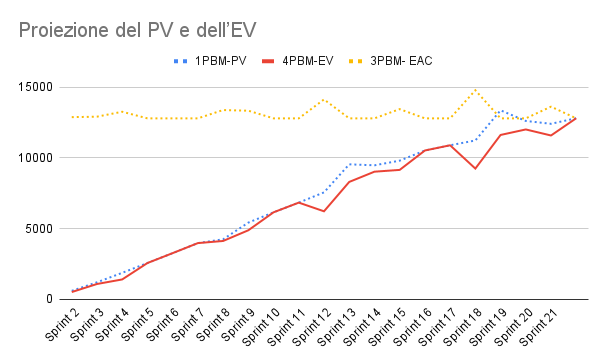
\includegraphics[width=0.8\textwidth]{../../img/pdq_charts/chart1-proiezionePVEV.png}
            \caption{Proiezione di PV ed EV}
        \end{figure}
        Dal grafico si può notare come Planned Value ed Earned Value quasi si sovrappongano. Questo denota una buona pianificazione ed aderenza da parte del gruppo. Inoltre si nota come convergano in modo abbastanza lineare al valore Estimate at Completion, il che suggerisce una distribuzione omogenea del lavoro nel corso delle settimane.

        \subsubsection{5PBM-AC - Actual Cost e 2PBM-ETC - Estimate to Complete}
        \begin{figure}[H]
            \centering
            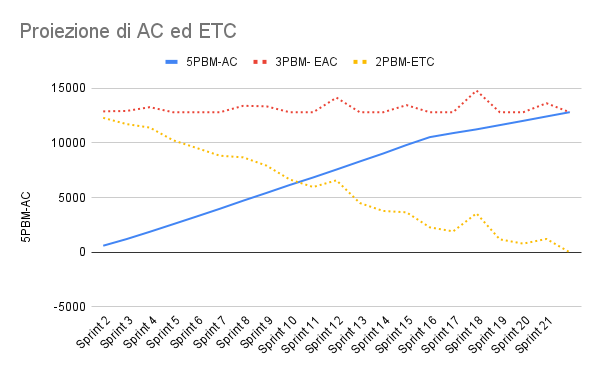
\includegraphics[width=0.8\textwidth]{../../img/pdq_charts/chart2-proiezioneACETC.png}
            \caption{Proiezione di AC e ETC}
        \end{figure}
        Dal grafico si osserva un progressivo aumento dell'Actual Cost, inversamente proporzionale al'Estimate to Complete, con un Estimate at Completion stabile nel tempo. Ciò implica una buona aderenza ai costi preventivati in fase di aggiudicazione.

        \subsubsection{6PBM-SV - Schedule Variance e 7PBM-CV - Cost Variance}
        \begin{figure}[H]
            \centering
            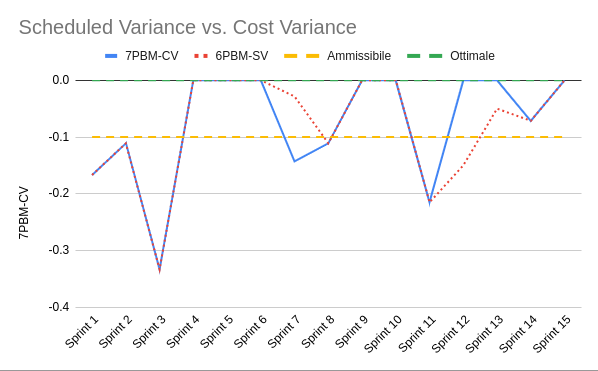
\includegraphics[width=0.8\textwidth]{../../img/pdq_charts/chart3-proiezioneSVCV.png}
            \caption{Proiezione di SV e CV}
        \end{figure}
        Il grafico evidenzia come Scheduled Variance e Cost Variance si sovrappongano quasi sempre, il che dimostra una buona capacità di programmare le attività e completarle per tempo.

        \subsubsection{3PBM-EAC - Estimated at Completion}
        \begin{figure}[H]
            \centering
            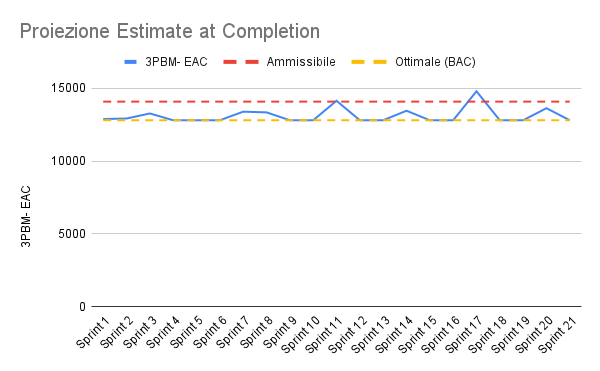
\includegraphics[width=0.8\textwidth]{../../img/pdq_charts/chart4-proiezioneEAC.png}
            \caption{Proiezione di EAC}
        \end{figure}
        Dal grafico si può vedere come il valore di Estimate at Completion coincida con il costo preventivato, ad eccezione di alcuni momenti critici in cui sfiora la soglia massima ammissibile per poi subito rientrare tra i valori ottimali.


    \subsection{Qualità processo di Documentazione}
        \subsubsection{1PSM-IG - Indice Gulpease}
        \begin{figure}[H]
            \centering
            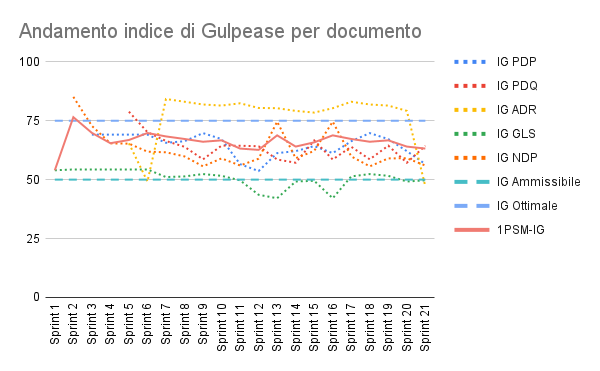
\includegraphics[width=0.8\textwidth]{../../img/pdq_charts/chart5-indiceGulpease.png}
            \caption{Indice di Gulpease per documento}
        \end{figure}
        Come si può vedere dal grafico l'indice di Gulpease si mantiene sempre tra il valore ammissibile e l'ottimale. Ciò è indice di una buona qualità della documentazione.


    \subsection{Qualità del processo di gestione della qualità}
        \subsubsection{7PSM-QMS - Metriche di Qualità Soddisfatte}
        \begin{figure}[H]
            \centering
            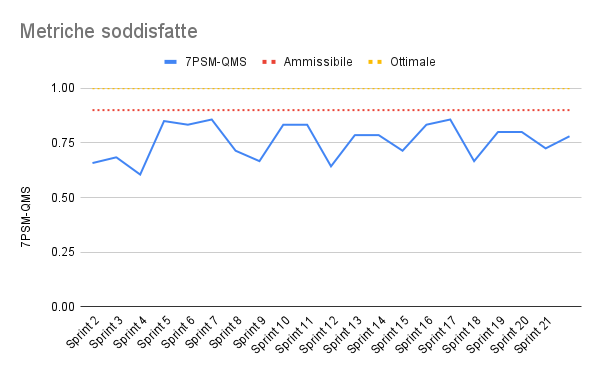
\includegraphics[width=0.8\textwidth]{../../img/pdq_charts/chart6-metricheSoddisfatte.png}
            \caption{Metriche di qualità soddisfatte}
        \end{figure}
        Come si può notare la quantità di metriche soddisfatte sono appena sotto il range ammissibile. Tuttavia nel calcolo del QMS sono considerate anche metriche legate al codice e a test su di esso. Considerando che il codice non è ancora stato sviluppato è naturale che questo valore sia basso.


    \subsection{Qualità del processo di pianificazione}
        \subsubsection{1POM-RSI - Requirements Stability Index}
        \begin{figure}[H]
            \centering
            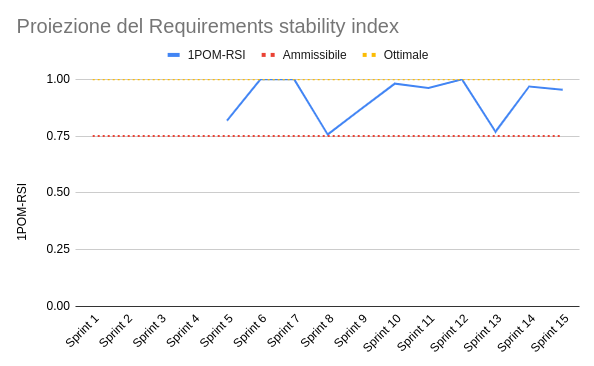
\includegraphics[width=0.8\textwidth]{../../img/pdq_charts/chart7-proiezioneRSI.png}
            \caption{Metriche di qualità soddisfatte}
        \end{figure}
        L'andamento del Requirements Stability Index mostra come i requisiti, dal momento della loro analisi, abbiano subito variazioni stabili e contenute entro i limiti previsti.

%%%%%%%%%%%%%%%%%%%%%%%%%%%%%%%%%%%%%%%%%%%%%%%%%%%%%%%%%%%%%%%%%%%%%%%%%%%%%%%%%%%

\newpage
\section{Iniziative di automiglioramento per la qualità}
\subsection{Introduzione}
In questa sezione vengono descritte le azioni intraprese per migliorare la qualità del prodotto e dei processi. 
Ogni iniziativa è stata identificata attraverso l’esperienza accumulata durante lo sviluppo del progetto, mano a mano che emergono problematiche specifiche. 
Essendo questa la nostra prima esperienza con un progetto di tale complessità, è stato necessario affrontare numerosi tentativi per capire come organizzarci e gestire le diverse attività in modo efficace. 
Durante il percorso, siamo riusciti a riconoscere i punti di forza e le aree di miglioramento nel nostro lavoro, individuando così gli aspetti su cui focalizzarci per ottimizzare il processo. 
Per ogni difficoltà riscontrata, sono riportati i seguenti dettagli:
\begin{itemize}
    \item La fase del progetto in cui si è verificato il problema;
    \item Descrizione del problema;
    \item Contromisura adottata per risolvere il problema evidenziato;
\end{itemize}

\subsection{Problemi Rilevati ed iniziative adottate}
\subsubsection{Presentazioni del diario di Bordo}
\begin{itemize}
    \item \textbf{Fase del Progetto:} Iniziale;
    \item \textbf{Descrizione:} Ogni settimana è richiesta una presentazione che illustri le attività svolte durante la settimana. È necessario preparare delle slide ed esporle di persona, ma per alcuni membri questo risulta difficoltoso a causa di impegni lavorativi o distanza. Nonostante una tabella che riportasse i ruoli settimanali di ciascun membro.
    \item \textbf{Contromisura:} Abbiamo deciso che i membri responsabili durante il periodo delle \textit{vacanze natalizie}, in cui non sono previste attività di diario di bordo, sostituiranno i colleghi che non possono presentare. In caso di diari di bordo online, saranno loro a presentare per primi.
\end{itemize}
\subsubsection{Organizzazione delle riunioni}
\begin{itemize}
    \item \textbf{Fase del Progetto:} Intermedia;
    \item \textbf{Descrizione:} In realtà siamo rimasti stupiti che questo problema non si sia presentato fin da subito, ma durante il mese di dicembre ci sono stati problemi sulle sprint interne con molti membri assenti, questo ha portato ad un rallentamento del lavoro anche per la discrepanza di conoscenze che ogni membro ha. A volte, alcuni membri non sapevano dove recuperare determinate informazioni o se i documenti fossero pronti. La situazione è peggiorata quando solo pochi membri si autoassegnavano le \textit{issue}.
    \item \textbf{Contromisura:} Abbiamo deciso di rendere la stesura dei verbali un'attività prioritaria da svolgere durante la riunione, cercando di completarla il più rapidamente possibile. Questo aiuta anche chi deve presentare il diario di bordo. Inoltre, per ogni \textit{issue} creata, abbiamo notificato tutti i membri tramite le piattaforme di comunicazione, in modo che tutti fossero consapevoli del lavoro da svolgere durante la sprint. Inoltre per evitare riunioni con pochi membri abbiamo preso in considerazione di essere più flessibili sull'orario delle riunioni settimanali.
\end{itemize}

\newpage
\subsection{Considerazioni Finali}
Fin da subito il nostro gruppo si è posto come obiettivo quello di dotarsi di un \textit{Way of Working} preciso e ben definito, pianificando ogni singola attività e prevedendo tutte le possibili difficoltà durante lo svolgimento del progetto.
Questo per cercare di prevenire i problemi e di affrontarli con contromisure efficaci. Alcuni problemi sono stati descritti in aula durante il corso, altri sono emersi confrontandoci con altri gruppi durante le attività di diario di bordo, mentre altri ancora li abbiamo affrontati direttamente nel nostro lavoro. Grazie ai consigli e ai suggerimenti esterni, siamo riusciti a implementare contromisure per risolverli o prevenirli fin dall'inizio."
Questo ha migliorato notevolmente la qualità del nostro lavoro e ci ha permesso di svolgere le varie attività in modo efficiente ed equo. Nonostante ciò siamo consapevoli che ci sono ancora molti aspetti su cui possiamo progredire e che ci sono molte iniziative di automiglioramento che possiamo adottare.
Siamo convinti che, continuando a lavorare con lo stesso impegno e determinazione, raggiungeremo risultati di qualità sempre più elevata.

\end{document}